% Options for packages loaded elsewhere
\PassOptionsToPackage{unicode}{hyperref}
\PassOptionsToPackage{hyphens}{url}
%
\documentclass[
]{article}
\usepackage{amsmath,amssymb}
\usepackage{lmodern}
\usepackage{iftex}
\ifPDFTeX
  \usepackage[T1]{fontenc}
  \usepackage[utf8]{inputenc}
  \usepackage{textcomp} % provide euro and other symbols
\else % if luatex or xetex
  \usepackage{unicode-math}
  \defaultfontfeatures{Scale=MatchLowercase}
  \defaultfontfeatures[\rmfamily]{Ligatures=TeX,Scale=1}
\fi
% Use upquote if available, for straight quotes in verbatim environments
\IfFileExists{upquote.sty}{\usepackage{upquote}}{}
\IfFileExists{microtype.sty}{% use microtype if available
  \usepackage[]{microtype}
  \UseMicrotypeSet[protrusion]{basicmath} % disable protrusion for tt fonts
}{}
\makeatletter
\@ifundefined{KOMAClassName}{% if non-KOMA class
  \IfFileExists{parskip.sty}{%
    \usepackage{parskip}
  }{% else
    \setlength{\parindent}{0pt}
    \setlength{\parskip}{6pt plus 2pt minus 1pt}}
}{% if KOMA class
  \KOMAoptions{parskip=half}}
\makeatother
\usepackage{xcolor}
\usepackage[margin=1in]{geometry}
\usepackage{color}
\usepackage{fancyvrb}
\newcommand{\VerbBar}{|}
\newcommand{\VERB}{\Verb[commandchars=\\\{\}]}
\DefineVerbatimEnvironment{Highlighting}{Verbatim}{commandchars=\\\{\}}
% Add ',fontsize=\small' for more characters per line
\usepackage{framed}
\definecolor{shadecolor}{RGB}{248,248,248}
\newenvironment{Shaded}{\begin{snugshade}}{\end{snugshade}}
\newcommand{\AlertTok}[1]{\textcolor[rgb]{0.94,0.16,0.16}{#1}}
\newcommand{\AnnotationTok}[1]{\textcolor[rgb]{0.56,0.35,0.01}{\textbf{\textit{#1}}}}
\newcommand{\AttributeTok}[1]{\textcolor[rgb]{0.77,0.63,0.00}{#1}}
\newcommand{\BaseNTok}[1]{\textcolor[rgb]{0.00,0.00,0.81}{#1}}
\newcommand{\BuiltInTok}[1]{#1}
\newcommand{\CharTok}[1]{\textcolor[rgb]{0.31,0.60,0.02}{#1}}
\newcommand{\CommentTok}[1]{\textcolor[rgb]{0.56,0.35,0.01}{\textit{#1}}}
\newcommand{\CommentVarTok}[1]{\textcolor[rgb]{0.56,0.35,0.01}{\textbf{\textit{#1}}}}
\newcommand{\ConstantTok}[1]{\textcolor[rgb]{0.00,0.00,0.00}{#1}}
\newcommand{\ControlFlowTok}[1]{\textcolor[rgb]{0.13,0.29,0.53}{\textbf{#1}}}
\newcommand{\DataTypeTok}[1]{\textcolor[rgb]{0.13,0.29,0.53}{#1}}
\newcommand{\DecValTok}[1]{\textcolor[rgb]{0.00,0.00,0.81}{#1}}
\newcommand{\DocumentationTok}[1]{\textcolor[rgb]{0.56,0.35,0.01}{\textbf{\textit{#1}}}}
\newcommand{\ErrorTok}[1]{\textcolor[rgb]{0.64,0.00,0.00}{\textbf{#1}}}
\newcommand{\ExtensionTok}[1]{#1}
\newcommand{\FloatTok}[1]{\textcolor[rgb]{0.00,0.00,0.81}{#1}}
\newcommand{\FunctionTok}[1]{\textcolor[rgb]{0.00,0.00,0.00}{#1}}
\newcommand{\ImportTok}[1]{#1}
\newcommand{\InformationTok}[1]{\textcolor[rgb]{0.56,0.35,0.01}{\textbf{\textit{#1}}}}
\newcommand{\KeywordTok}[1]{\textcolor[rgb]{0.13,0.29,0.53}{\textbf{#1}}}
\newcommand{\NormalTok}[1]{#1}
\newcommand{\OperatorTok}[1]{\textcolor[rgb]{0.81,0.36,0.00}{\textbf{#1}}}
\newcommand{\OtherTok}[1]{\textcolor[rgb]{0.56,0.35,0.01}{#1}}
\newcommand{\PreprocessorTok}[1]{\textcolor[rgb]{0.56,0.35,0.01}{\textit{#1}}}
\newcommand{\RegionMarkerTok}[1]{#1}
\newcommand{\SpecialCharTok}[1]{\textcolor[rgb]{0.00,0.00,0.00}{#1}}
\newcommand{\SpecialStringTok}[1]{\textcolor[rgb]{0.31,0.60,0.02}{#1}}
\newcommand{\StringTok}[1]{\textcolor[rgb]{0.31,0.60,0.02}{#1}}
\newcommand{\VariableTok}[1]{\textcolor[rgb]{0.00,0.00,0.00}{#1}}
\newcommand{\VerbatimStringTok}[1]{\textcolor[rgb]{0.31,0.60,0.02}{#1}}
\newcommand{\WarningTok}[1]{\textcolor[rgb]{0.56,0.35,0.01}{\textbf{\textit{#1}}}}
\usepackage{graphicx}
\makeatletter
\def\maxwidth{\ifdim\Gin@nat@width>\linewidth\linewidth\else\Gin@nat@width\fi}
\def\maxheight{\ifdim\Gin@nat@height>\textheight\textheight\else\Gin@nat@height\fi}
\makeatother
% Scale images if necessary, so that they will not overflow the page
% margins by default, and it is still possible to overwrite the defaults
% using explicit options in \includegraphics[width, height, ...]{}
\setkeys{Gin}{width=\maxwidth,height=\maxheight,keepaspectratio}
% Set default figure placement to htbp
\makeatletter
\def\fps@figure{htbp}
\makeatother
\setlength{\emergencystretch}{3em} % prevent overfull lines
\providecommand{\tightlist}{%
  \setlength{\itemsep}{0pt}\setlength{\parskip}{0pt}}
\setcounter{secnumdepth}{-\maxdimen} % remove section numbering
\ifLuaTeX
  \usepackage{selnolig}  % disable illegal ligatures
\fi
\IfFileExists{bookmark.sty}{\usepackage{bookmark}}{\usepackage{hyperref}}
\IfFileExists{xurl.sty}{\usepackage{xurl}}{} % add URL line breaks if available
\urlstyle{same} % disable monospaced font for URLs
\hypersetup{
  pdftitle={HUDM6026 Final Project},
  pdfauthor={Chenguang Pan \& Seng Lei},
  hidelinks,
  pdfcreator={LaTeX via pandoc}}

\title{HUDM6026 Final Project}
\author{Chenguang Pan \& Seng Lei}
\date{April 28, 2023}

\begin{document}
\maketitle

\hypertarget{introduction}{%
\subsection{1.0 Introduction}\label{introduction}}

High School Longitudinal Study of 2009(HSLS:09) is a nationally
representative, longitudinal study of 23,000+ ninth graders from 944
schools in 2009. It provides comprehensive information about student's
background, academic performance in both high school and college,
personal attitudes towards study and school, etc. Therefore, this
current project decided to work on the HSLS:09 open dataset.

Based on the HSLS09 open data, we investigate the potential relationship
between ninth-grader's mathematics foundation and future achievement in
STEM fields. To accomplish this objective, a simple linear regression
model was employed, which allowed for the estimation of the effect of
math proficiency on overall GPA in STEM courses throughout high school.
The standardized mathematics assessment of algebraic reasoning,
administered during the first semester of grade 9, was utilized to
measure students' mathematical foundation at the onset of high school.
In turn, the overall GPA in STEM courses was used as a metric of
academic performance in STEM subjects throughout the high school years.

After some data cleaning, we kept 199,948 observations for analysis. The
simple linear model is: \[y_i = \beta_0 + \beta_1\times x_i + e_i ,\]
where \(y_i\) is the estimated individual outcome for overall STEM GPA,
\(x_i\) is the student's mathematics assessment score, and \(e_i\) is
the residual.

\hypertarget{population-data-descriptions}{%
\subsection{2.0 Population data
descriptions}\label{population-data-descriptions}}

As a simulated study, we treated cleaned dataset as the population,
\emph{N}=19948. The mean and standard deviation for the dependent
variable are 2.440 and .934. And 51.250 and 10.031 for the predictor.
The correlation coefficient between these two variables is .567.

\begin{Shaded}
\begin{Highlighting}[]
\SpecialCharTok{\textgreater{}}\NormalTok{ model\_lm }\OtherTok{\textless{}{-}} \FunctionTok{lm}\NormalTok{(X3TGPASTEM }\SpecialCharTok{\textasciitilde{}}\NormalTok{ X1TXMTSCOR, }\AttributeTok{data =}\NormalTok{ hsls\_sub)}
\SpecialCharTok{\textgreater{}} \FunctionTok{summary}\NormalTok{(model\_lm)}

\NormalTok{Call}\SpecialCharTok{:}
\FunctionTok{lm}\NormalTok{(}\AttributeTok{formula =}\NormalTok{ X3TGPASTEM }\SpecialCharTok{\textasciitilde{}}\NormalTok{ X1TXMTSCOR, }\AttributeTok{data =}\NormalTok{ hsls\_sub)}

\NormalTok{Residuals}\SpecialCharTok{:}
\NormalTok{     Min       1Q   Median       3Q      Max }
\SpecialCharTok{{-}}\FloatTok{2.82822} \SpecialCharTok{{-}}\FloatTok{0.50345}  \FloatTok{0.05364}  \FloatTok{0.55167}  \FloatTok{2.70153} 

\NormalTok{Coefficients}\SpecialCharTok{:}
\NormalTok{             Estimate Std. Error t value }\FunctionTok{Pr}\NormalTok{(}\SpecialCharTok{\textgreater{}}\ErrorTok{|}\NormalTok{t}\SpecialCharTok{|}\NormalTok{)    }
\NormalTok{(Intercept) }\SpecialCharTok{{-}}\FloatTok{0.264846}   \FloatTok{0.028358}  \SpecialCharTok{{-}}\FloatTok{9.339}   \SpecialCharTok{\textless{}}\FloatTok{2e{-}16} \SpecialCharTok{**}\ErrorTok{*}
\NormalTok{X1TXMTSCOR   }\FloatTok{0.052792}   \FloatTok{0.000543}  \FloatTok{97.220}   \SpecialCharTok{\textless{}}\FloatTok{2e{-}16} \SpecialCharTok{**}\ErrorTok{*}
\SpecialCharTok{{-}{-}{-}}
\NormalTok{Signif. codes}\SpecialCharTok{:}  \DecValTok{0} \StringTok{\textquotesingle{}***\textquotesingle{}} \FloatTok{0.001} \StringTok{\textquotesingle{}**\textquotesingle{}} \FloatTok{0.01} \StringTok{\textquotesingle{}*\textquotesingle{}} \FloatTok{0.05} \StringTok{\textquotesingle{}.\textquotesingle{}} \FloatTok{0.1} \StringTok{\textquotesingle{} \textquotesingle{}} \DecValTok{1}

\NormalTok{Residual standard error}\SpecialCharTok{:} \FloatTok{0.7693}\NormalTok{ on }\DecValTok{19946}\NormalTok{ degrees of freedom}
\NormalTok{Multiple R}\SpecialCharTok{{-}}\NormalTok{squared}\SpecialCharTok{:}  \FloatTok{0.3215}\NormalTok{,    Adjusted R}\SpecialCharTok{{-}}\NormalTok{squared}\SpecialCharTok{:}  \FloatTok{0.3215} 
\NormalTok{F}\SpecialCharTok{{-}}\NormalTok{statistic}\SpecialCharTok{:}  \DecValTok{9452}\NormalTok{ on }\DecValTok{1}\NormalTok{ and }\DecValTok{19946}\NormalTok{ DF,  p}\SpecialCharTok{{-}}\NormalTok{value}\SpecialCharTok{:} \ErrorTok{\textless{}} \FloatTok{2.2e{-}16}
\end{Highlighting}
\end{Shaded}

The simple linear regression model presented that the overall model can
explain the 32.15\% of the variance in outcome, \(F(1,19946)=9452\),
\(p < .001\). One score increase in 9th grader's math assessment will be
associated with .053 increase in overall STEM GPA and this relation is
statistically significant, \(\beta_1=.053\), \(p <.001\). The expected
value of overall STEM GPA (i.e., \(\beta_0\)) when student gets zero in
math assessment is \(-.265\), \(p <.001\). The negative GPA does not
make any sense, but we ignored this issue and move on the study.

\hypertarget{writing-r-functions}{%
\subsection{3.0 Writing R functions}\label{writing-r-functions}}

\begin{Shaded}
\begin{Highlighting}[]
\SpecialCharTok{\textgreater{}}\NormalTok{ dat\_gen }\OtherTok{\textless{}{-}} \ControlFlowTok{function}\NormalTok{(}\AttributeTok{size=} \DecValTok{500}\NormalTok{,  }\CommentTok{\# smaple size}
\SpecialCharTok{+}\NormalTok{                     betas,      }\CommentTok{\# a numeric array of betas}
\SpecialCharTok{+}\NormalTok{                     iv\_mean,    }\CommentTok{\# predictor\textquotesingle{}s mean}
\SpecialCharTok{+}\NormalTok{                     iv\_var,     }\CommentTok{\# predictor\textquotesingle{}s variance}
\SpecialCharTok{+}\NormalTok{                     error\_sd)\{  }\CommentTok{\# residuals\textquotesingle{} sd}
\SpecialCharTok{+}   \CommentTok{\# data mainly are generated from a normal distribution \textasciitilde{} N(iv\_mean, iv\_sd)}
\SpecialCharTok{+}\NormalTok{   X }\OtherTok{\textless{}{-}} \FunctionTok{rnorm}\NormalTok{(size, }\AttributeTok{mean =}\NormalTok{ iv\_mean, }\AttributeTok{sd=} \FunctionTok{sqrt}\NormalTok{(iv\_var))}
\SpecialCharTok{+}\NormalTok{   X\_aug }\OtherTok{\textless{}{-}} \FunctionTok{cbind}\NormalTok{(}\DecValTok{1}\NormalTok{, X)}
\SpecialCharTok{+}   \CommentTok{\# residuals are generated from \textasciitilde{}N(0, sd)}
\SpecialCharTok{+}\NormalTok{   Error }\OtherTok{\textless{}{-}} \FunctionTok{rnorm}\NormalTok{(size, }\AttributeTok{mean=}\DecValTok{0}\NormalTok{, }\AttributeTok{sd=}\NormalTok{error\_sd)}
\SpecialCharTok{+}   \CommentTok{\# based on the parameters to generate the outcomes}
\SpecialCharTok{+}\NormalTok{   Y }\OtherTok{\textless{}{-}}\NormalTok{ X\_aug }\SpecialCharTok{\%*\%} \FunctionTok{as.matrix}\NormalTok{(betas) }\SpecialCharTok{+}\NormalTok{ Error}
\SpecialCharTok{+}\NormalTok{   out }\OtherTok{\textless{}{-}} \FunctionTok{cbind}\NormalTok{(Y, X)}
\SpecialCharTok{+}   \FunctionTok{colnames}\NormalTok{(out) }\OtherTok{\textless{}{-}} \FunctionTok{c}\NormalTok{(}\StringTok{"Y"}\NormalTok{, }\StringTok{"X1"}\NormalTok{)}
\SpecialCharTok{+}   \FunctionTok{return}\NormalTok{(}\FunctionTok{as.data.frame}\NormalTok{(out))}
\SpecialCharTok{+}\NormalTok{ \}}
\end{Highlighting}
\end{Shaded}

The data generation function takes the sample size, regression
coefficients, predictors' mean and variance, and the standard deviation
of residual as input. It returns a simulated dataset in
\texttt{dataframe} format with the outcome in the first column and
predictor in the second.

\begin{Shaded}
\begin{Highlighting}[]
\SpecialCharTok{\textgreater{}}\NormalTok{ reg }\OtherTok{\textless{}{-}} \ControlFlowTok{function}\NormalTok{(ds) \{}
\SpecialCharTok{+}\NormalTok{   x }\OtherTok{\textless{}{-}} \FunctionTok{as.matrix}\NormalTok{(ds[,}\DecValTok{2}\NormalTok{])}
\SpecialCharTok{+}\NormalTok{   y }\OtherTok{\textless{}{-}} \FunctionTok{as.matrix}\NormalTok{(ds[,}\DecValTok{1}\NormalTok{])}
\SpecialCharTok{+}\NormalTok{   y\_cen }\OtherTok{\textless{}{-}} \FunctionTok{apply}\NormalTok{(y, }\DecValTok{2}\NormalTok{, }\ControlFlowTok{function}\NormalTok{(x) x}\SpecialCharTok{{-}}\FunctionTok{mean}\NormalTok{(x))}
\SpecialCharTok{+}\NormalTok{   x\_cen }\OtherTok{\textless{}{-}} \FunctionTok{apply}\NormalTok{(x, }\DecValTok{2}\NormalTok{, }\ControlFlowTok{function}\NormalTok{(x) x}\SpecialCharTok{{-}}\FunctionTok{mean}\NormalTok{(x))}
\SpecialCharTok{+}   \CommentTok{\# the OLS method}
\SpecialCharTok{+}\NormalTok{   b1 }\OtherTok{\textless{}{-}} \FunctionTok{sum}\NormalTok{(x\_cen}\SpecialCharTok{*}\NormalTok{y\_cen)}\SpecialCharTok{/}\FunctionTok{sum}\NormalTok{(x\_cen}\SpecialCharTok{\^{}}\DecValTok{2}\NormalTok{)}
\SpecialCharTok{+}\NormalTok{   b0 }\OtherTok{\textless{}{-}} \FunctionTok{mean}\NormalTok{(y }\SpecialCharTok{{-}}\NormalTok{ x}\SpecialCharTok{*}\NormalTok{b1)}
\SpecialCharTok{+}\NormalTok{   y\_hat }\OtherTok{\textless{}{-}}\NormalTok{ b0 }\SpecialCharTok{+}\NormalTok{ x}\SpecialCharTok{*}\NormalTok{b1}
\SpecialCharTok{+}\NormalTok{   sse }\OtherTok{\textless{}{-}} \FunctionTok{sum}\NormalTok{((y}\SpecialCharTok{{-}}\NormalTok{y\_hat)}\SpecialCharTok{\^{}}\DecValTok{2}\NormalTok{)}
\SpecialCharTok{+}\NormalTok{   sig\_sq }\OtherTok{\textless{}{-}}\NormalTok{ sse}\SpecialCharTok{/}\NormalTok{(}\FunctionTok{nrow}\NormalTok{(x)}\SpecialCharTok{{-}}\DecValTok{2}\NormalTok{)}
\SpecialCharTok{+}   \CommentTok{\# the alternative method}
\SpecialCharTok{+}\NormalTok{   b1\_a }\OtherTok{\textless{}{-}} \FunctionTok{sum}\NormalTok{(y\_cen}\SpecialCharTok{/}\NormalTok{x\_cen)}\SpecialCharTok{/}\FunctionTok{nrow}\NormalTok{(x)}
\SpecialCharTok{+}\NormalTok{   b0\_a }\OtherTok{\textless{}{-}} \FunctionTok{mean}\NormalTok{(y }\SpecialCharTok{{-}}\NormalTok{ x}\SpecialCharTok{*}\NormalTok{b1\_a)}
\SpecialCharTok{+}\NormalTok{   y\_hat\_a }\OtherTok{\textless{}{-}}\NormalTok{ b0\_a }\SpecialCharTok{+}\NormalTok{ x}\SpecialCharTok{*}\NormalTok{b1\_a}
\SpecialCharTok{+}\NormalTok{   sse\_a }\OtherTok{\textless{}{-}} \FunctionTok{sum}\NormalTok{((y}\SpecialCharTok{{-}}\NormalTok{y\_hat\_a)}\SpecialCharTok{\^{}}\DecValTok{2}\NormalTok{)}
\SpecialCharTok{+}\NormalTok{   sig\_sq\_a }\OtherTok{\textless{}{-}}\NormalTok{ sse\_a}\SpecialCharTok{/}\FunctionTok{nrow}\NormalTok{(x)}
\SpecialCharTok{+}\NormalTok{   out\_ }\OtherTok{\textless{}{-}} \FunctionTok{cbind}\NormalTok{(b0, b1, sig\_sq, b0\_a, b1\_a,sig\_sq\_a)}
\SpecialCharTok{+}   \FunctionTok{return}\NormalTok{(out\_)}
\SpecialCharTok{+}\NormalTok{ \}}
\end{Highlighting}
\end{Shaded}

The estimation function takes the simulated data frame as input, and
returns the estimated \(\beta_0\), \(\beta_1\), residual's variance
\(\sigma^2\) from both least square and alternative methods.

\hypertarget{monte-carlo-simulation}{%
\subsection{4.0 Monte Carlo Simulation}\label{monte-carlo-simulation}}

The basic idea behind the Monte Carlo simulation is that one can draw a
large number of random samples from a probability distribution
representing the population being studied, and then these samples are
used to estimate its statistical properties. This project used Monte
Carlo method to draw 1000 random samples with the size of 40 by using
the \texttt{dat\_gen()} function above.

\begin{Shaded}
\begin{Highlighting}[]
\SpecialCharTok{\textgreater{}}\NormalTok{ R }\OtherTok{\textless{}{-}} \DecValTok{1000}
\SpecialCharTok{\textgreater{}} \FunctionTok{set.seed}\NormalTok{(}\DecValTok{666}\NormalTok{)}
\SpecialCharTok{\textgreater{}} \CommentTok{\# randomly generate 1000 samples}
\ErrorTok{\textgreater{}}\NormalTok{ dat\_list }\OtherTok{\textless{}{-}} \FunctionTok{replicate}\NormalTok{(}\AttributeTok{n =}\NormalTok{ R,}
\SpecialCharTok{+}                       \AttributeTok{expr =} \FunctionTok{dat\_gen}\NormalTok{(}\AttributeTok{size =} \DecValTok{40}\NormalTok{,}
\SpecialCharTok{+}                                      \AttributeTok{betas =} \FunctionTok{c}\NormalTok{(}\SpecialCharTok{{-}}\FloatTok{0.265}\NormalTok{,}\FloatTok{0.053}\NormalTok{),}
\SpecialCharTok{+}                                      \AttributeTok{iv\_mean =} \FloatTok{51.24985}\NormalTok{, }\AttributeTok{iv\_var =} \FloatTok{100.6209}\NormalTok{,}
\SpecialCharTok{+}                                      \AttributeTok{error\_sd =} \FloatTok{0.7693}\NormalTok{),}
\SpecialCharTok{+}                       \AttributeTok{simplify =} \ConstantTok{FALSE}\NormalTok{)}
\SpecialCharTok{\textgreater{}} \CommentTok{\# estimated the simple regression model on each sample}
\ErrorTok{\textgreater{}}\NormalTok{ estimates }\OtherTok{\textless{}{-}} \FunctionTok{sapply}\NormalTok{(}\AttributeTok{X =}\NormalTok{ dat\_list,}
\SpecialCharTok{+}                     \AttributeTok{FUN =}\NormalTok{ reg,}
\SpecialCharTok{+}                     \AttributeTok{simplify =} \ConstantTok{TRUE}\NormalTok{)}
\SpecialCharTok{\textgreater{}}\NormalTok{ estimates }\OtherTok{\textless{}{-}} \FunctionTok{t}\NormalTok{(estimates)}
\SpecialCharTok{\textgreater{}} \FunctionTok{colnames}\NormalTok{(estimates) }\OtherTok{\textless{}{-}} \FunctionTok{c}\NormalTok{(}\StringTok{"b0"}\NormalTok{, }\StringTok{"b1"}\NormalTok{, }\StringTok{"sig\_sq"}\NormalTok{, }\StringTok{"b0\_a"}\NormalTok{, }\StringTok{"b1\_a"}\NormalTok{, }\StringTok{"sig\_sq\_a"}\NormalTok{)}
\SpecialCharTok{\textgreater{}} 
\ErrorTok{\textgreater{}} \CommentTok{\# write a function to calculate the estimates}
\ErrorTok{\textgreater{}}\NormalTok{ est\_out }\OtherTok{\textless{}{-}} \ControlFlowTok{function}\NormalTok{(esti\_mat, size)\{}
\SpecialCharTok{+}   \CommentTok{\# to calculate the MSE}
\SpecialCharTok{+}   \CommentTok{\# first to make a parameter matrix in shape of the estimates matrix}
\SpecialCharTok{+}\NormalTok{   theta\_m }\OtherTok{\textless{}{-}} \FunctionTok{matrix}\NormalTok{(}\FunctionTok{c}\NormalTok{(}\SpecialCharTok{{-}}\FloatTok{0.265}\NormalTok{, }\FloatTok{0.053}\NormalTok{,}\FloatTok{0.7693}\NormalTok{), }\FunctionTok{nrow}\NormalTok{(esti\_mat),}\DecValTok{6}\NormalTok{ , }\AttributeTok{byrow =}\NormalTok{ T)}
\SpecialCharTok{+}   \CommentTok{\# use the estimates matrix minus the parameter matrix}
\SpecialCharTok{+}\NormalTok{   est\_cent }\OtherTok{\textless{}{-}}\NormalTok{esti\_mat}\SpecialCharTok{{-}}\NormalTok{theta\_m}
\SpecialCharTok{+}   \CommentTok{\# use apply to get the mse for each estimates}
\SpecialCharTok{+}\NormalTok{   estimates\_hat\_mean }\OtherTok{\textless{}{-}} \FunctionTok{round}\NormalTok{(}\FunctionTok{apply}\NormalTok{(esti\_mat,}\DecValTok{2}\NormalTok{,mean),}\DecValTok{3}\NormalTok{)}
\SpecialCharTok{+}\NormalTok{   estimates\_hat\_var }\OtherTok{\textless{}{-}} \FunctionTok{round}\NormalTok{(}\FunctionTok{apply}\NormalTok{(esti\_mat,}\DecValTok{2}\NormalTok{,var),}\DecValTok{3}\NormalTok{)}
\SpecialCharTok{+}\NormalTok{   estimates\_hat\_se }\OtherTok{\textless{}{-}} \FunctionTok{round}\NormalTok{(}\FunctionTok{apply}\NormalTok{(esti\_mat,}\DecValTok{2}\NormalTok{,}\ControlFlowTok{function}\NormalTok{(x) }\FunctionTok{sd}\NormalTok{(x)}\SpecialCharTok{/}\FunctionTok{sqrt}\NormalTok{(size)),}\DecValTok{3}\NormalTok{)}
\SpecialCharTok{+}\NormalTok{   estimates\_mse }\OtherTok{\textless{}{-}} \FunctionTok{round}\NormalTok{(}\FunctionTok{apply}\NormalTok{(est\_cent,}\DecValTok{2}\NormalTok{,}\ControlFlowTok{function}\NormalTok{(x) }\FunctionTok{sum}\NormalTok{(x}\SpecialCharTok{\^{}}\DecValTok{2}\NormalTok{)}\SpecialCharTok{/}\NormalTok{size),}\DecValTok{3}\NormalTok{)}
\SpecialCharTok{+}\NormalTok{   results }\OtherTok{\textless{}{-}} \FunctionTok{rbind}\NormalTok{(estimates\_hat\_mean,estimates\_hat\_var,}
\SpecialCharTok{+}\NormalTok{                    estimates\_hat\_se,estimates\_mse)}
\SpecialCharTok{+}   \FunctionTok{rownames}\NormalTok{(results) }\OtherTok{\textless{}{-}} \FunctionTok{c}\NormalTok{(}\StringTok{"Mean"}\NormalTok{, }\StringTok{"Variance"}\NormalTok{,}\StringTok{"SE"}\NormalTok{, }\StringTok{"MSE"}\NormalTok{)}
\SpecialCharTok{+}\NormalTok{   results\_trans }\OtherTok{\textless{}{-}} \FunctionTok{as.data.frame}\NormalTok{(}\FunctionTok{t}\NormalTok{(results))}
\SpecialCharTok{+}   \CommentTok{\# add a column to calculate the bias}
\SpecialCharTok{+}\NormalTok{   par\_m }\OtherTok{\textless{}{-}} \FunctionTok{matrix}\NormalTok{(}\FunctionTok{c}\NormalTok{(}\SpecialCharTok{{-}}\FloatTok{0.265}\NormalTok{, }\FloatTok{0.053}\NormalTok{,}\FloatTok{0.7693}\NormalTok{), }\DecValTok{6}\NormalTok{,}\DecValTok{1}\NormalTok{)}
\SpecialCharTok{+}\NormalTok{   results\_trans}\SpecialCharTok{$}\NormalTok{Bias }\OtherTok{\textless{}{-}}\NormalTok{ results\_trans}\SpecialCharTok{$}\NormalTok{Mean }\SpecialCharTok{{-}}\NormalTok{ par\_m}
\SpecialCharTok{+}\NormalTok{   results\_trans}\SpecialCharTok{$}\NormalTok{Parameter }\OtherTok{\textless{}{-}}\NormalTok{ par\_m}
\SpecialCharTok{+}\NormalTok{   results\_trans }\OtherTok{\textless{}{-}}\NormalTok{ results\_trans[,}\FunctionTok{c}\NormalTok{(}\DecValTok{6}\NormalTok{,}\DecValTok{1}\NormalTok{,}\DecValTok{3}\NormalTok{,}\DecValTok{2}\NormalTok{,}\DecValTok{5}\NormalTok{,}\DecValTok{4}\NormalTok{)]}
\SpecialCharTok{+}   \FunctionTok{return}\NormalTok{(results\_trans)}
\SpecialCharTok{+}\NormalTok{ \}}
\SpecialCharTok{\textgreater{}}\NormalTok{ (mc\_out }\OtherTok{\textless{}{-}} \FunctionTok{est\_out}\NormalTok{(estimates, R))}
\NormalTok{         Parameter    Mean     SE   Variance     Bias        MSE}
\NormalTok{b0         }\SpecialCharTok{{-}}\FloatTok{0.2650}  \SpecialCharTok{{-}}\FloatTok{0.265}  \FloatTok{0.020}      \FloatTok{0.415}   \FloatTok{0.0000}      \FloatTok{0.415}
\NormalTok{b1          }\FloatTok{0.0530}   \FloatTok{0.053}  \FloatTok{0.000}      \FloatTok{0.000}   \FloatTok{0.0000}      \FloatTok{0.000}
\NormalTok{sig\_sq      }\FloatTok{0.7693}   \FloatTok{0.585}  \FloatTok{0.004}      \FloatTok{0.017}  \SpecialCharTok{{-}}\FloatTok{0.1843}      \FloatTok{0.051}
\NormalTok{b0\_a       }\SpecialCharTok{{-}}\FloatTok{0.2650}  \SpecialCharTok{{-}}\FloatTok{5.143}  \FloatTok{1.887}   \FloatTok{3558.920}  \SpecialCharTok{{-}}\FloatTok{4.8780}   \FloatTok{3579.161}
\NormalTok{b1\_a        }\FloatTok{0.0530}   \FloatTok{0.146}  \FloatTok{0.036}      \FloatTok{1.317}   \FloatTok{0.0930}      \FloatTok{1.324}
\NormalTok{sig\_sq\_a    }\FloatTok{0.7693} \FloatTok{121.727} \FloatTok{29.594} \FloatTok{875788.198} \FloatTok{120.9577} \FloatTok{889543.113}
\end{Highlighting}
\end{Shaded}

\hypertarget{bootstrap-method}{%
\subsection{5.0 Bootstrap method}\label{bootstrap-method}}

The bootstrap method is a statistical technique that involves the
repeated sampling with replacement from the original data to obtain
estimates of variability and uncertainty of a statistic of interest.
Specifically, the statistic is computed on each of the resamples, and
the resulting distribution is used to calculate confidence intervals or
conduct hypothesis tests. Since we have a single sample of 40
observations in this context, the bootstrap method is proposed to be
applied to the row indices of the original dataset. Each resample would
be created based on the shuffled indices of the original data, thus
allowing for the generation of multiple estimates of the statistic of
interest.

The R function for bootstrap is as follows.

\begin{Shaded}
\begin{Highlighting}[]
\SpecialCharTok{\textgreater{}} \CommentTok{\# generate a single dataset}
\ErrorTok{\textgreater{}}\NormalTok{ data\_b }\OtherTok{\textless{}{-}}\FunctionTok{dat\_gen}\NormalTok{(}\AttributeTok{size =} \DecValTok{40}\NormalTok{,}\AttributeTok{betas =} \FunctionTok{c}\NormalTok{(}\SpecialCharTok{{-}}\FloatTok{0.265}\NormalTok{,}\FloatTok{0.053}\NormalTok{),}
\SpecialCharTok{+}                 \AttributeTok{iv\_mean =} \FloatTok{51.24985}\NormalTok{, }\AttributeTok{iv\_var =} \FloatTok{100.6209}\NormalTok{,}
\SpecialCharTok{+}                 \AttributeTok{error\_sd =} \FloatTok{0.7693}\NormalTok{)}
\SpecialCharTok{\textgreater{}} \CommentTok{\# run bootstrapping on this single dataset}
\ErrorTok{\textgreater{}}\NormalTok{ B }\OtherTok{=} \DecValTok{1000}
\SpecialCharTok{\textgreater{}} \CommentTok{\# shuffle the 1:40 index rather than data\_b}
\ErrorTok{\textgreater{}}\NormalTok{ boot\_index }\OtherTok{\textless{}{-}} \FunctionTok{replicate}\NormalTok{(}\AttributeTok{n=}\NormalTok{B,}
\SpecialCharTok{+}                        \AttributeTok{expr =} \FunctionTok{sample}\NormalTok{(}\DecValTok{1}\SpecialCharTok{:}\DecValTok{40}\NormalTok{, }\DecValTok{40}\NormalTok{, }\ConstantTok{TRUE}\NormalTok{),}
\SpecialCharTok{+}                        \AttributeTok{simplify =} \ConstantTok{FALSE}\NormalTok{)}
\SpecialCharTok{\textgreater{}} \CommentTok{\# use the bootstrapped indices to extracted the data}
\ErrorTok{\textgreater{}}\NormalTok{ boot\_samp }\OtherTok{\textless{}{-}} \FunctionTok{list}\NormalTok{()}
\SpecialCharTok{\textgreater{}} \ControlFlowTok{for}\NormalTok{ (i }\ControlFlowTok{in} \DecValTok{1}\SpecialCharTok{:}\DecValTok{1000}\NormalTok{) \{}
\SpecialCharTok{+}\NormalTok{   boot\_unit }\OtherTok{\textless{}{-}}\NormalTok{ data\_b[boot\_index[[i]],]}
\SpecialCharTok{+}\NormalTok{   boot\_samp[[i]] }\OtherTok{\textless{}{-}}\NormalTok{ boot\_unit}
\SpecialCharTok{+}\NormalTok{ \}}
\SpecialCharTok{\textgreater{}}\NormalTok{ estimates }\OtherTok{\textless{}{-}} \FunctionTok{sapply}\NormalTok{(}\AttributeTok{X =}\NormalTok{ boot\_samp,}
\SpecialCharTok{+}                     \AttributeTok{FUN =}\NormalTok{ reg,}
\SpecialCharTok{+}                     \AttributeTok{simplify =} \ConstantTok{TRUE}\NormalTok{)}
\SpecialCharTok{\textgreater{}}\NormalTok{ estimates }\OtherTok{\textless{}{-}} \FunctionTok{t}\NormalTok{(estimates)}
\SpecialCharTok{\textgreater{}} \FunctionTok{colnames}\NormalTok{(estimates) }\OtherTok{\textless{}{-}} \FunctionTok{c}\NormalTok{(}\StringTok{"b0"}\NormalTok{, }\StringTok{"b1"}\NormalTok{, }\StringTok{"sig\_sq"}\NormalTok{, }\StringTok{"b0\_a"}\NormalTok{, }\StringTok{"b1\_a"}\NormalTok{, }\StringTok{"sig\_sq\_a"}\NormalTok{)}
\SpecialCharTok{\textgreater{}} 
\ErrorTok{\textgreater{}}\NormalTok{ (bs\_out}\OtherTok{\textless{}{-}}\FunctionTok{est\_out}\NormalTok{(estimates, B))}
\NormalTok{         Parameter     Mean       SE     Variance      Bias          MSE}
\NormalTok{b0         }\SpecialCharTok{{-}}\FloatTok{0.2650}   \SpecialCharTok{{-}}\FloatTok{0.568}    \FloatTok{0.019} \FloatTok{3.670000e{-}01}   \SpecialCharTok{{-}}\FloatTok{0.3030} \FloatTok{4.580000e{-}01}
\NormalTok{b1          }\FloatTok{0.0530}    \FloatTok{0.058}    \FloatTok{0.000} \FloatTok{0.000000e+00}    \FloatTok{0.0050} \FloatTok{0.000000e+00}
\NormalTok{sig\_sq      }\FloatTok{0.7693}    \FloatTok{0.477}    \FloatTok{0.004} \FloatTok{1.200000e{-}02}   \SpecialCharTok{{-}}\FloatTok{0.2923} \FloatTok{9.800000e{-}02}
\NormalTok{b0\_a       }\SpecialCharTok{{-}}\FloatTok{0.2650}    \FloatTok{2.819}    \FloatTok{7.072} \FloatTok{5.000976e+04}    \FloatTok{3.0840} \FloatTok{4.996926e+04}
\NormalTok{b1\_a        }\FloatTok{0.0530}   \SpecialCharTok{{-}}\FloatTok{0.010}    \FloatTok{0.139} \FloatTok{1.922100e+01}   \SpecialCharTok{{-}}\FloatTok{0.0630} \FloatTok{1.920600e+01}
\NormalTok{sig\_sq\_a    }\FloatTok{0.7693} \FloatTok{3220.335} \FloatTok{2961.135} \FloatTok{8.768318e+09} \FloatTok{3219.5657} \FloatTok{8.769915e+09}
\end{Highlighting}
\end{Shaded}

\hypertarget{jackknife-method}{%
\subsection{6.0 Jackknife method}\label{jackknife-method}}

The jackknife method is a statistical technique to estimate the bias and
variance of a statistic by systematically leaving out one observation at
a time from the dataset, creating a series of ``jackknife samples''. By
recalculating the statistic of interest on each of these samples, we can
obtain an approximation of the distribution of the statistic, and use it
to estimate its bias and standard error. In the present context, we
applied the jackknife method to the same 40-observation dataset.

\begin{Shaded}
\begin{Highlighting}[]
\SpecialCharTok{\textgreater{}}\NormalTok{ jack\_list }\OtherTok{\textless{}{-}} \FunctionTok{list}\NormalTok{()}
\SpecialCharTok{\textgreater{}} \ControlFlowTok{for}\NormalTok{ (i }\ControlFlowTok{in} \DecValTok{1}\SpecialCharTok{:}\DecValTok{40}\NormalTok{) \{}
\SpecialCharTok{+}   \CommentTok{\# each round drop the ith observation}
\SpecialCharTok{+}\NormalTok{   data\_loov }\OtherTok{\textless{}{-}}\NormalTok{ data\_b[}\SpecialCharTok{{-}}\NormalTok{i,]}
\SpecialCharTok{+}   \CommentTok{\# make a list to load each jacknife sample}
\SpecialCharTok{+}\NormalTok{   jack\_list[[i]] }\OtherTok{\textless{}{-}}\NormalTok{ data\_loov}
\SpecialCharTok{+}\NormalTok{ \}}
\SpecialCharTok{\textgreater{}} 
\ErrorTok{\textgreater{}}\NormalTok{ estimates }\OtherTok{\textless{}{-}} \FunctionTok{sapply}\NormalTok{(}\AttributeTok{X =}\NormalTok{ jack\_list,}
\SpecialCharTok{+}                     \AttributeTok{FUN =}\NormalTok{ reg,}
\SpecialCharTok{+}                     \AttributeTok{simplify =} \ConstantTok{TRUE}\NormalTok{)}
\SpecialCharTok{\textgreater{}}\NormalTok{ estimates }\OtherTok{\textless{}{-}} \FunctionTok{t}\NormalTok{(estimates) }
\SpecialCharTok{\textgreater{}} \CommentTok{\# this is a 40 x 6 matrix}
\ErrorTok{\textgreater{}} \FunctionTok{colnames}\NormalTok{(estimates) }\OtherTok{\textless{}{-}} \FunctionTok{c}\NormalTok{(}\StringTok{"b0"}\NormalTok{, }\StringTok{"b1"}\NormalTok{, }\StringTok{"sig\_sq"}\NormalTok{, }\StringTok{"b0\_a"}\NormalTok{, }\StringTok{"b1\_a"}\NormalTok{, }\StringTok{"sig\_sq\_a"}\NormalTok{)}
\SpecialCharTok{\textgreater{}} 
\ErrorTok{\textgreater{}} \CommentTok{\# since the population parameter is known, we use them directly}
\ErrorTok{\textgreater{}}\NormalTok{ (jn\_out}\OtherTok{\textless{}{-}}\FunctionTok{est\_out}\NormalTok{(estimates, }\DecValTok{40}\NormalTok{))}
\NormalTok{         Parameter   Mean     SE   Variance    Bias        MSE}
\NormalTok{b0         }\SpecialCharTok{{-}}\FloatTok{0.2650} \SpecialCharTok{{-}}\FloatTok{0.533}  \FloatTok{0.016}      \FloatTok{0.010} \SpecialCharTok{{-}}\FloatTok{0.2680}      \FloatTok{0.082}
\NormalTok{b1          }\FloatTok{0.0530}  \FloatTok{0.057}  \FloatTok{0.000}      \FloatTok{0.000}  \FloatTok{0.0040}      \FloatTok{0.000}
\NormalTok{sig\_sq      }\FloatTok{0.7693}  \FloatTok{0.510}  \FloatTok{0.003}      \FloatTok{0.000} \SpecialCharTok{{-}}\FloatTok{0.2593}      \FloatTok{0.068}
\NormalTok{b0\_a       }\SpecialCharTok{{-}}\FloatTok{0.2650} \SpecialCharTok{{-}}\FloatTok{4.347}  \FloatTok{6.444}   \FloatTok{1661.026} \SpecialCharTok{{-}}\FloatTok{4.0820}   \FloatTok{1636.160}
\NormalTok{b1\_a        }\FloatTok{0.0530}  \FloatTok{0.133}  \FloatTok{0.129}      \FloatTok{0.667}  \FloatTok{0.0800}      \FloatTok{0.657}
\NormalTok{sig\_sq\_a    }\FloatTok{0.7693} \FloatTok{96.400} \FloatTok{87.796} \FloatTok{308322.929} \FloatTok{95.6307} \FloatTok{309760.012}
\end{Highlighting}
\end{Shaded}

One should notice that the population information is available in this
simulated study. Therefore, we chose to not use the plug-in principle to
estimate the bias or MSE.

\hypertarget{comparing-the-results}{%
\subsection{7.0 Comparing the results}\label{comparing-the-results}}

\emph{Table 1} combines the outcomes from all three methods.

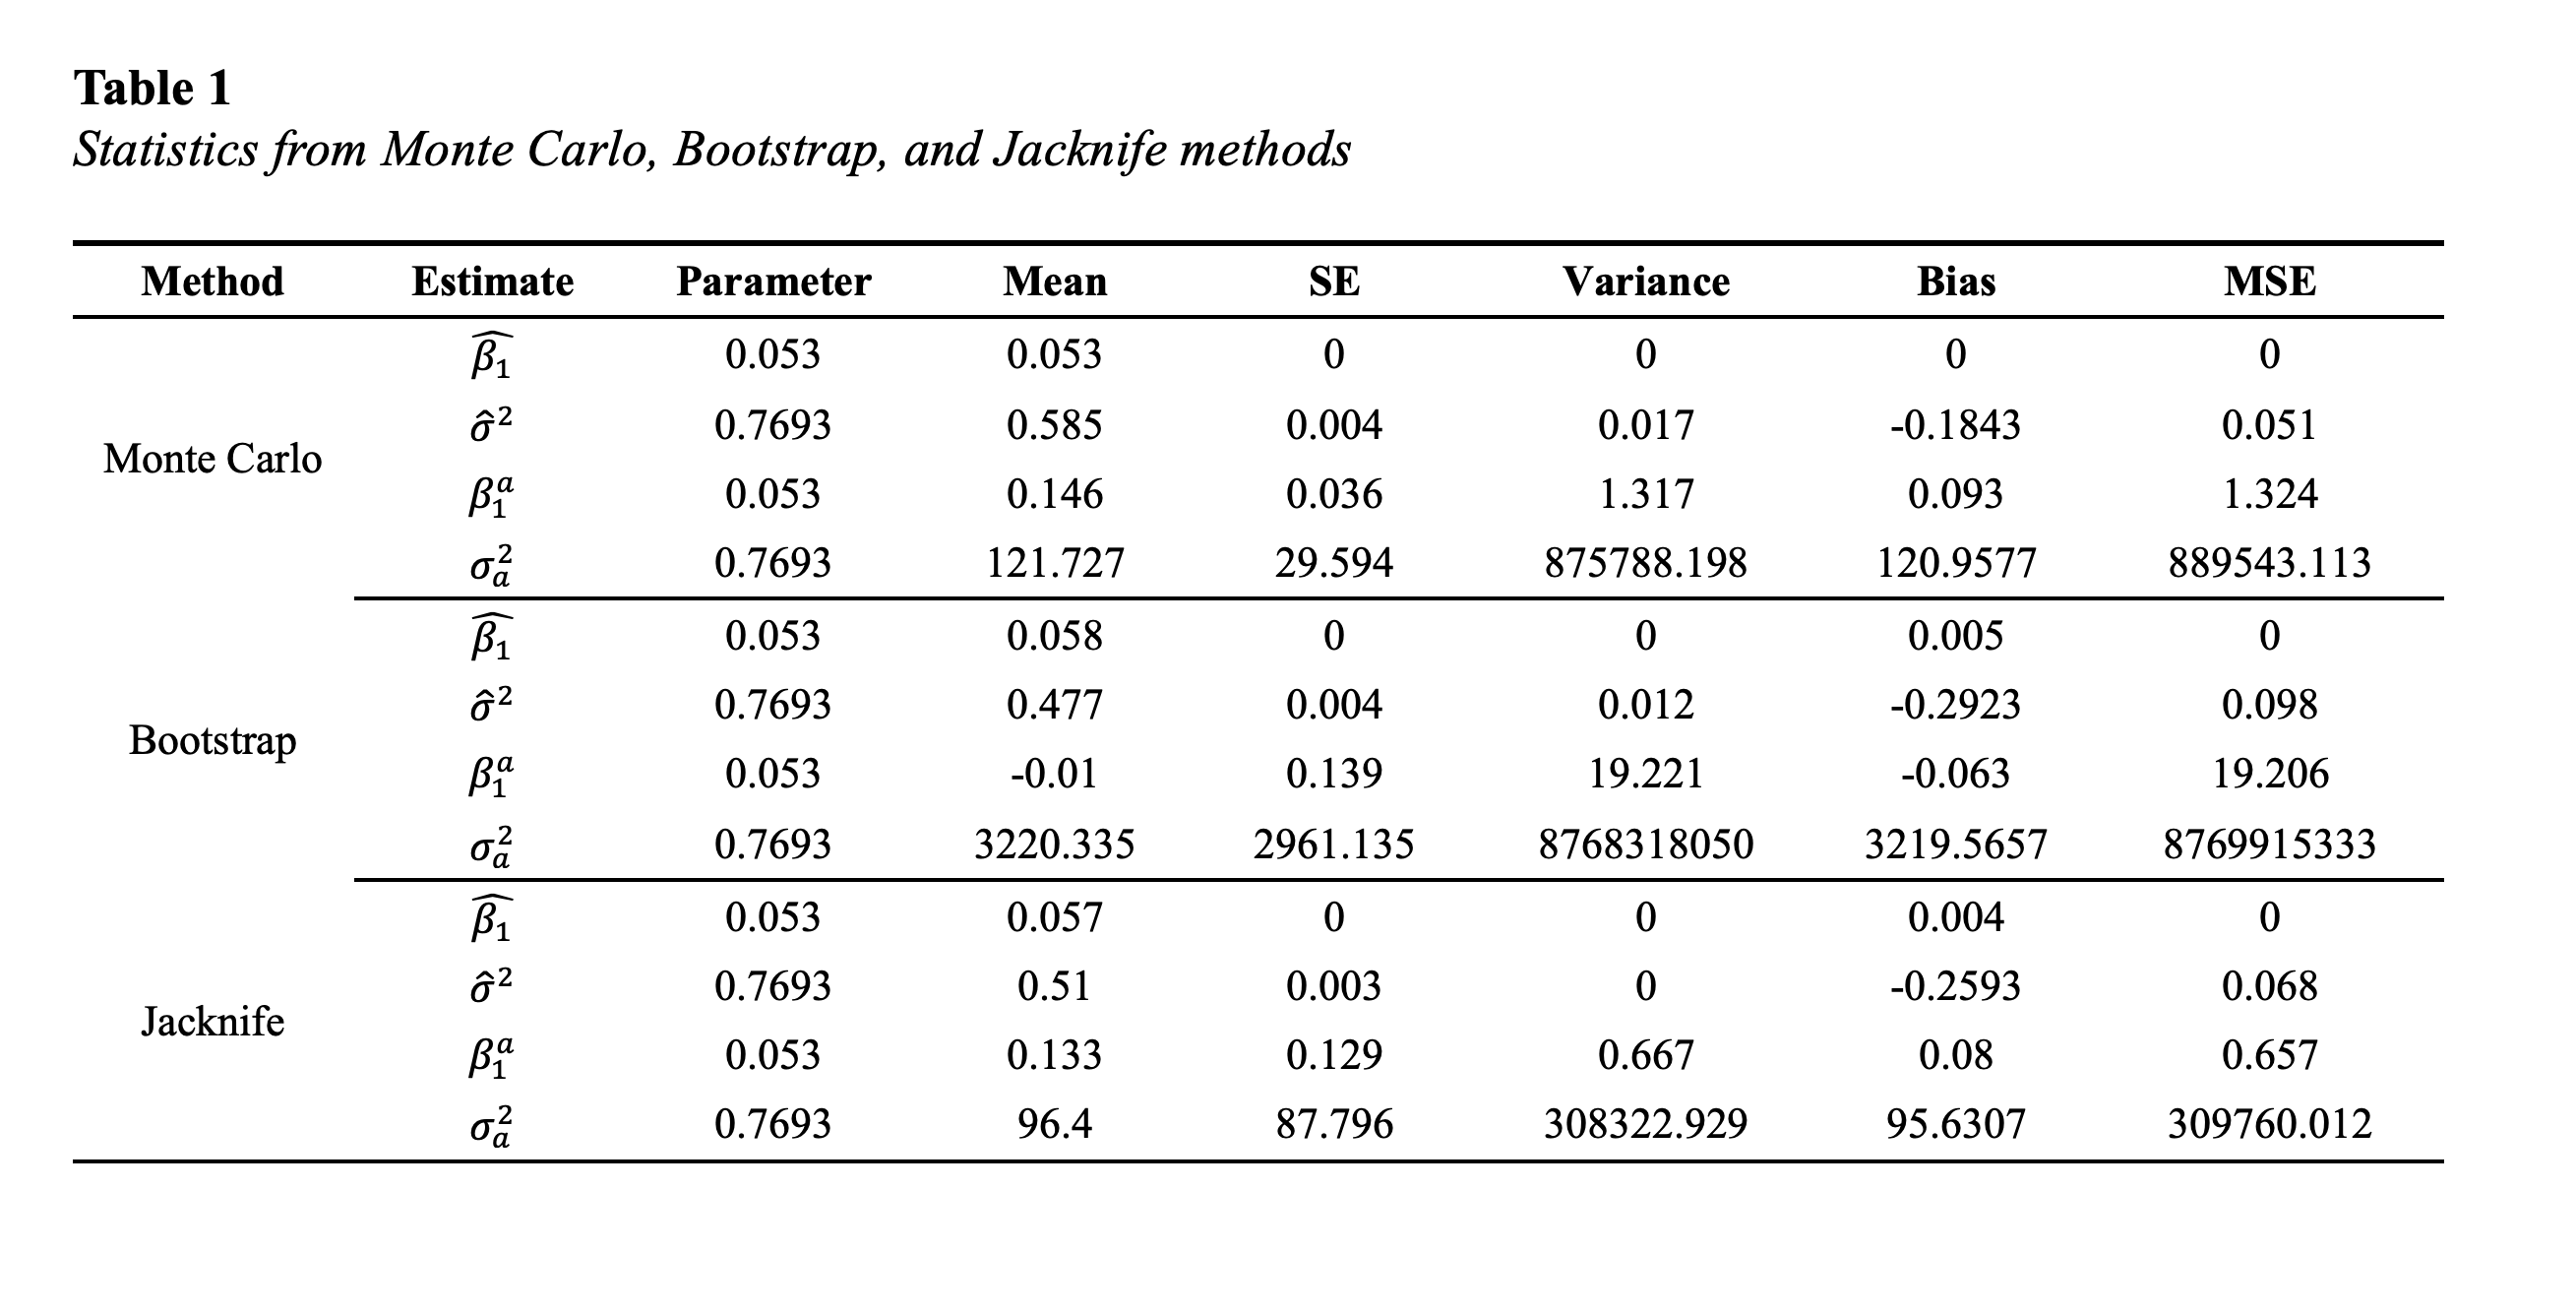
\includegraphics{"~/Desktop/PhD_Learning/HUDM6026 Computational Statistics/HUDM6026_Final_Project/03_outputs/04_output_APA.png"}

For the estimation of both \(\beta_1\) and \(\sigma^2\), the OLS method
shows lower variance,bias, and therefore lower MSE than the alternative
way in all data simulation methods. The alternative estimator of the
\(\sigma_2\) is much larger than it under the OLS method. One of the
reason is the alternative way is sensitive to the outliers during the
resampling process. Comparing to the average value, the median looks
more reasonable.

\hypertarget{discussion}{%
\subsection{8.0 Discussion}\label{discussion}}

\hypertarget{the-ols-method-versus-the-alternative-method}{%
\subsubsection{8.1 The OLS method versus the alternative
method}\label{the-ols-method-versus-the-alternative-method}}

OLS estimator of \(\beta_1\) is \[\hat\beta_1 = \frac{S_{xy}}{S_x^2},\]
Which can write
into:\[\hat\beta_1 =\frac{\sum_{i=1}^{n}(x_i-\bar{x})(y_i-\bar{y})}{\sum_{i=1}^{n}(x_i-\bar{x})^2} = \sum_{i=1}^{n}\frac{(x_i-\bar{x})^2}{\sum_{i=1}^{n}(x_i-\bar{x})^2}\frac{(y_i-\bar{y})}{(x_i-\bar{x})}. \]

Since this term is the slope of the line between point i to the center
point of the data \[\frac{(y_i-\bar{y})}{(x_i-\bar{x})},\] we can
conclude \(\beta_1\) is a weighted average of slope of the line that
connects the i-th point to the average of all points, the weight is
determined by the distance of x to mean of x. The longer distance would
be weighted more since small changes in its position will affect the
slope connecting it to the center point more than closer points. We
expect estimated Beta1 in OLS would be close to true Beta.

\[\hat\sigma^2 = \frac{SSE}{n-2}\] This is an unbiased estimate of the
population \(\sigma^2\) So when we generate a large number of samples
and the average should be close to the true \(\sigma^2.\)

The alternative estimator of \(\beta_1\) is
\[\beta_1^a = \frac{1}{n}\sum_{i=1}^{n}\frac{(y_i-\bar{y})}{(x_i-\bar{x})}.\]

\(\beta_1\) is the average slope for all the points in the sample, each
point is equally weighted compared to OLS. This estimator would be less
sensitive to the points far to the center. So it can not capture the
change in y efficiently when the point is far from the center. Then the
estimated Beta1 in the alternative method would be less close to true
Beta.

\[\sigma^2_a = \frac{SSE}{n}\]

The alternative estimator for sample variance is a biased estimator
which will underestimate the true \(\sigma^2\). But since the SSE was
based on Alternative \(\beta_1\), it would depend on the estimated value
of y heavily. And since the Alternative estimator for Beta1 would be
less accurate, the sample variance would be larger than expected.

\hypertarget{monte-carlo-vs.-bootstrap-vs.-jackknife}{%
\subsubsection{8.2 Monte Carlo vs.~Bootstrap
vs.~Jackknife}\label{monte-carlo-vs.-bootstrap-vs.-jackknife}}

From the result table and compared to the theory, it basically matches
our guessing. Using the OLS approach, the \(\beta_1\) estimation was
very close to the true beta, with 0 standard error and variance. Which
means in every sample we generated, the estimator of \(\beta_1\) is
identical. The result in Bootstrap and Jackknife is slightly different
from true beta which can be due to the replacement of the points in each
sample in bootstrap and leaving-one-out for Jackknife.

As for the Alternative approach, we could find these estimated
\(\beta_1\) are not even close to the true beta, which leads to a huge
variance in alternative estimator for variance.

\hypertarget{the-optimal-procedure}{%
\subsubsection{8.3 The optimal procedure}\label{the-optimal-procedure}}

Monte Carlo seems to have a better bias, variance and SEM since it was
generating data from the sample distribution, while jackknife and
bootstrap are using the real observed data.

\hypertarget{pros-and-cons-for-the-three-procedures}{%
\subsubsection{8.4 Pros and cons for the three
procedures}\label{pros-and-cons-for-the-three-procedures}}

Jackknife's pros is more friendly to computational power, but the cons
it might be less accurate than Monte Carlo and bootstrap since it can
only provide n samples for studying. So when sample size is small this
is not a good resampling method.

Bootstrap provides sample distributions with replacement, the pros is it
provide a good estimates of uncertainty. The cons is if we did not
generate a big enough number of samples,the information from one point
might be more heavy than other points in the estimation. So the
bootstrap is sensitive to number of samples we generate. Another problem
is if the real sample does not represent the population, we can not
obtain any useful estimation towards the population, since bootstrap
only repeat the observation in the sample. Finally, bootstrap is
computational intensive.

Monte Carlo can be useful when we have a correct belief about the
population distribution. It is a good way to estimate uncertainty. The
cons is very sensitive to the input of generating process and cost much
computational power.

\end{document}
